% Created by tikzDevice version 0.12 on 2019-04-11 07:16:37
% !TEX encoding = UTF-8 Unicode
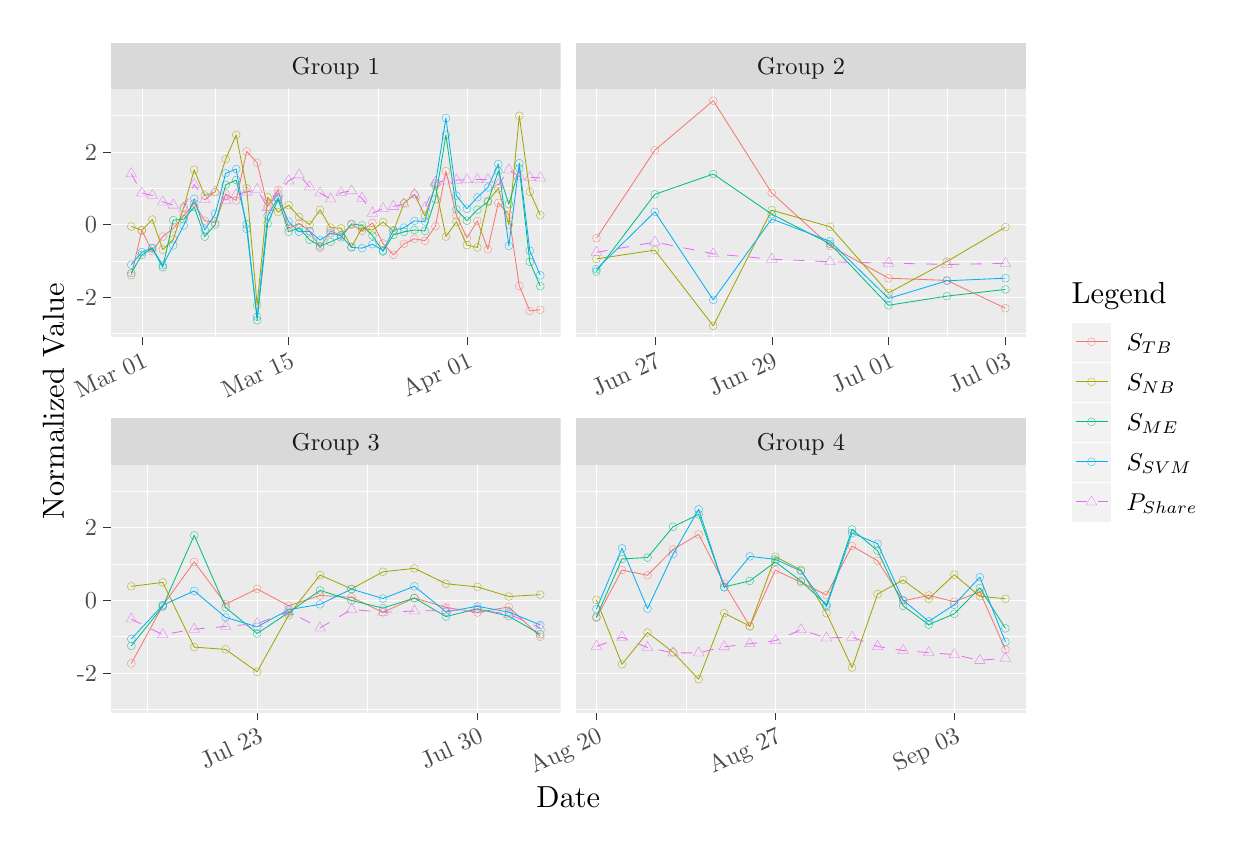
\begin{tikzpicture}[x=1pt,y=1pt]
\definecolor{fillColor}{RGB}{255,255,255}
\path[use as bounding box,fill=fillColor,fill opacity=0.00] (0,0) rectangle (433.62,289.08);
\begin{scope}
\path[clip] (  0.00,  0.00) rectangle (433.62,289.08);
\definecolor{drawColor}{RGB}{255,255,255}
\definecolor{fillColor}{RGB}{255,255,255}

\path[draw=drawColor,line width= 0.1pt,line join=round,line cap=round,fill=fillColor] (  0.00,  0.00) rectangle (433.62,289.08);
\end{scope}
\begin{scope}
\path[clip] ( 30.06,177.26) rectangle (192.62,266.77);
\definecolor{fillColor}{gray}{0.92}

\path[fill=fillColor] ( 30.06,177.26) rectangle (192.62,266.77);
\definecolor{drawColor}{RGB}{255,255,255}

\path[draw=drawColor,line width= 0.1pt,line join=round] ( 30.06,178.61) --
	(192.62,178.61);

\path[draw=drawColor,line width= 0.1pt,line join=round] ( 30.06,204.86) --
	(192.62,204.86);

\path[draw=drawColor,line width= 0.1pt,line join=round] ( 30.06,231.10) --
	(192.62,231.10);

\path[draw=drawColor,line width= 0.1pt,line join=round] ( 30.06,257.34) --
	(192.62,257.34);

\path[draw=drawColor,line width= 0.1pt,line join=round] ( 67.76,177.26) --
	( 67.76,266.77);

\path[draw=drawColor,line width= 0.1pt,line join=round] (126.50,177.26) --
	(126.50,266.77);

\path[draw=drawColor,line width= 0.1pt,line join=round] (185.23,177.26) --
	(185.23,266.77);

\path[draw=drawColor,line width= 0.1pt,line join=round] ( 30.06,191.73) --
	(192.62,191.73);

\path[draw=drawColor,line width= 0.1pt,line join=round] ( 30.06,217.98) --
	(192.62,217.98);

\path[draw=drawColor,line width= 0.1pt,line join=round] ( 30.06,244.22) --
	(192.62,244.22);

\path[draw=drawColor,line width= 0.1pt,line join=round] ( 41.23,177.26) --
	( 41.23,266.77);

\path[draw=drawColor,line width= 0.1pt,line join=round] ( 94.29,177.26) --
	( 94.29,266.77);

\path[draw=drawColor,line width= 0.1pt,line join=round] (158.71,177.26) --
	(158.71,266.77);
\definecolor{drawColor}{RGB}{248,118,109}

\path[draw=drawColor,line width= 0.3pt,line join=round] ( 37.44,199.59) --
	( 41.23,215.79) --
	( 45.02,208.33) --
	( 48.81,213.59) --
	( 52.60,216.55) --
	( 56.39,221.17) --
	( 60.18,225.63) --
	( 63.97,219.31) --
	( 67.76,218.69) --
	( 71.55,228.95) --
	( 75.34,226.66) --
	( 79.13,244.40) --
	( 82.92,240.24) --
	( 86.71,224.49) --
	( 90.50,230.43) --
	( 94.29,216.64) --
	( 98.08,218.34) --
	(101.86,215.63) --
	(105.65,209.49) --
	(109.44,215.58) --
	(113.23,214.09) --
	(117.02,217.88) --
	(120.81,215.66) --
	(124.60,218.51) --
	(128.39,211.13) --
	(132.18,206.96) --
	(135.97,210.97) --
	(139.76,212.78) --
	(143.55,212.09) --
	(147.34,217.28) --
	(151.13,237.22) --
	(154.92,221.27) --
	(158.71,213.10) --
	(162.49,219.25) --
	(166.28,209.00) --
	(170.07,225.80) --
	(173.86,221.43) --
	(177.65,195.75) --
	(181.44,186.71) --
	(185.23,187.17);
\definecolor{drawColor}{RGB}{163,165,0}

\path[draw=drawColor,line width= 0.3pt,line join=round] ( 37.44,217.26) --
	( 41.23,215.87) --
	( 45.02,219.74) --
	( 48.81,208.87) --
	( 52.60,212.59) --
	( 56.39,224.16) --
	( 60.18,237.73) --
	( 63.97,228.41) --
	( 67.76,229.67) --
	( 71.55,241.59) --
	( 75.34,250.32) --
	( 79.13,231.07) --
	( 82.92,188.83) --
	( 86.71,227.82) --
	( 90.50,222.41) --
	( 94.29,224.92) --
	( 98.08,220.67) --
	(101.86,217.90) --
	(105.65,223.26) --
	(109.44,216.82) --
	(113.23,216.61) --
	(117.02,209.83) --
	(120.81,216.67) --
	(124.60,215.93) --
	(128.39,218.84) --
	(132.18,215.52) --
	(135.97,225.66) --
	(139.76,228.85) --
	(143.55,221.05) --
	(147.34,231.98) --
	(151.13,213.57) --
	(154.92,218.95) --
	(158.71,210.52) --
	(162.49,209.64) --
	(166.28,226.40) --
	(170.07,230.99) --
	(173.86,217.92) --
	(177.65,257.24) --
	(181.44,229.81) --
	(185.23,221.30);
\definecolor{drawColor}{RGB}{0,191,125}

\path[draw=drawColor,line width= 0.3pt,line join=round] ( 37.44,200.37) --
	( 41.23,206.97) --
	( 45.02,209.30) --
	( 48.81,202.48) --
	( 52.60,219.53) --
	( 56.39,219.86) --
	( 60.18,224.27) --
	( 63.97,213.57) --
	( 67.76,217.90) --
	( 71.55,232.28) --
	( 75.34,234.02) --
	( 79.13,218.05) --
	( 82.92,183.36) --
	( 86.71,218.35) --
	( 90.50,227.13) --
	( 94.29,215.35) --
	( 98.08,216.72) --
	(101.86,212.45) --
	(105.65,210.14) --
	(109.44,211.66) --
	(113.23,213.32) --
	(117.02,218.18) --
	(120.81,217.62) --
	(124.60,213.94) --
	(128.39,208.21) --
	(132.18,214.24) --
	(135.97,215.26) --
	(139.76,215.96) --
	(143.55,215.63) --
	(147.34,227.15) --
	(151.13,250.33) --
	(154.92,223.42) --
	(158.71,219.30) --
	(162.49,223.31) --
	(166.28,226.10) --
	(170.07,237.19) --
	(173.86,225.30) --
	(177.65,238.27) --
	(181.44,204.47) --
	(185.23,195.66);
\definecolor{drawColor}{RGB}{0,176,246}

\path[draw=drawColor,line width= 0.3pt,line join=round] ( 37.44,203.44) --
	( 41.23,207.94) --
	( 45.02,209.48) --
	( 48.81,203.18) --
	( 52.60,210.39) --
	( 56.39,217.59) --
	( 60.18,227.25) --
	( 63.97,216.02) --
	( 67.76,221.78) --
	( 71.55,236.47) --
	( 75.34,238.00) --
	( 79.13,216.40) --
	( 82.92,184.61) --
	( 86.71,221.08) --
	( 90.50,227.65) --
	( 94.29,218.97) --
	( 98.08,215.33) --
	(101.86,215.47) --
	(105.65,212.31) --
	(109.44,214.82) --
	(113.23,213.90) --
	(117.02,209.68) --
	(120.81,209.41) --
	(124.60,210.82) --
	(128.39,208.56) --
	(132.18,215.87) --
	(135.97,216.79) --
	(139.76,219.25) --
	(143.55,219.05) --
	(147.34,232.70) --
	(151.13,256.41) --
	(154.92,228.37) --
	(158.71,223.62) --
	(162.49,227.77) --
	(166.28,231.32) --
	(170.07,239.80) --
	(173.86,210.21) --
	(177.65,240.09) --
	(181.44,208.48) --
	(185.23,199.60);
\definecolor{drawColor}{RGB}{231,107,243}

\path[draw=drawColor,line width= 0.3pt,dash pattern=on 4pt off 4pt ,line join=round] ( 37.44,236.30) --
	( 41.23,229.36) --
	( 45.02,228.46) --
	( 48.81,226.14) --
	( 52.60,224.98) --
	( 56.39,223.83) --
	( 60.18,232.44) --
	( 63.97,226.91) --
	( 67.76,229.74) --
	( 71.55,226.78) --
	( 75.34,228.71) --
	( 79.13,229.68) --
	( 82.92,230.64) --
	( 86.71,224.08) --
	( 90.50,229.10) --
	( 94.29,233.73) --
	( 98.08,235.91) --
	(101.86,231.54) --
	(105.65,229.36) --
	(109.44,227.17) --
	(113.23,229.48) --
	(117.02,230.13) --
	(120.81,227.43) --
	(124.60,222.03) --
	(128.39,223.70) --
	(132.18,224.53) --
	(135.97,225.37) --
	(139.76,228.84) --
	(143.55,223.96) --
	(147.34,233.21) --
	(151.13,233.73) --
	(154.92,233.98) --
	(158.71,234.11) --
	(162.49,234.18) --
	(166.28,234.24) --
	(170.07,232.31) --
	(173.86,237.71) --
	(177.65,235.27) --
	(181.44,234.95) --
	(185.23,234.79);
\definecolor{drawColor}{RGB}{248,118,109}

\path[draw=drawColor,line width= 0.1pt,line join=round,line cap=round] ( 37.44,199.59) circle (  1.43);

\path[draw=drawColor,line width= 0.1pt,line join=round,line cap=round] ( 41.23,215.79) circle (  1.43);

\path[draw=drawColor,line width= 0.1pt,line join=round,line cap=round] ( 45.02,208.33) circle (  1.43);

\path[draw=drawColor,line width= 0.1pt,line join=round,line cap=round] ( 48.81,213.59) circle (  1.43);

\path[draw=drawColor,line width= 0.1pt,line join=round,line cap=round] ( 52.60,216.55) circle (  1.43);

\path[draw=drawColor,line width= 0.1pt,line join=round,line cap=round] ( 56.39,221.17) circle (  1.43);

\path[draw=drawColor,line width= 0.1pt,line join=round,line cap=round] ( 60.18,225.63) circle (  1.43);

\path[draw=drawColor,line width= 0.1pt,line join=round,line cap=round] ( 63.97,219.31) circle (  1.43);

\path[draw=drawColor,line width= 0.1pt,line join=round,line cap=round] ( 67.76,218.69) circle (  1.43);

\path[draw=drawColor,line width= 0.1pt,line join=round,line cap=round] ( 71.55,228.95) circle (  1.43);

\path[draw=drawColor,line width= 0.1pt,line join=round,line cap=round] ( 75.34,226.66) circle (  1.43);

\path[draw=drawColor,line width= 0.1pt,line join=round,line cap=round] ( 79.13,244.40) circle (  1.43);

\path[draw=drawColor,line width= 0.1pt,line join=round,line cap=round] ( 82.92,240.24) circle (  1.43);

\path[draw=drawColor,line width= 0.1pt,line join=round,line cap=round] ( 86.71,224.49) circle (  1.43);

\path[draw=drawColor,line width= 0.1pt,line join=round,line cap=round] ( 90.50,230.43) circle (  1.43);

\path[draw=drawColor,line width= 0.1pt,line join=round,line cap=round] ( 94.29,216.64) circle (  1.43);

\path[draw=drawColor,line width= 0.1pt,line join=round,line cap=round] ( 98.08,218.34) circle (  1.43);

\path[draw=drawColor,line width= 0.1pt,line join=round,line cap=round] (101.86,215.63) circle (  1.43);

\path[draw=drawColor,line width= 0.1pt,line join=round,line cap=round] (105.65,209.49) circle (  1.43);

\path[draw=drawColor,line width= 0.1pt,line join=round,line cap=round] (109.44,215.58) circle (  1.43);

\path[draw=drawColor,line width= 0.1pt,line join=round,line cap=round] (113.23,214.09) circle (  1.43);

\path[draw=drawColor,line width= 0.1pt,line join=round,line cap=round] (117.02,217.88) circle (  1.43);

\path[draw=drawColor,line width= 0.1pt,line join=round,line cap=round] (120.81,215.66) circle (  1.43);

\path[draw=drawColor,line width= 0.1pt,line join=round,line cap=round] (124.60,218.51) circle (  1.43);

\path[draw=drawColor,line width= 0.1pt,line join=round,line cap=round] (128.39,211.13) circle (  1.43);

\path[draw=drawColor,line width= 0.1pt,line join=round,line cap=round] (132.18,206.96) circle (  1.43);

\path[draw=drawColor,line width= 0.1pt,line join=round,line cap=round] (135.97,210.97) circle (  1.43);

\path[draw=drawColor,line width= 0.1pt,line join=round,line cap=round] (139.76,212.78) circle (  1.43);

\path[draw=drawColor,line width= 0.1pt,line join=round,line cap=round] (143.55,212.09) circle (  1.43);

\path[draw=drawColor,line width= 0.1pt,line join=round,line cap=round] (147.34,217.28) circle (  1.43);

\path[draw=drawColor,line width= 0.1pt,line join=round,line cap=round] (151.13,237.22) circle (  1.43);

\path[draw=drawColor,line width= 0.1pt,line join=round,line cap=round] (154.92,221.27) circle (  1.43);

\path[draw=drawColor,line width= 0.1pt,line join=round,line cap=round] (158.71,213.10) circle (  1.43);

\path[draw=drawColor,line width= 0.1pt,line join=round,line cap=round] (162.49,219.25) circle (  1.43);

\path[draw=drawColor,line width= 0.1pt,line join=round,line cap=round] (166.28,209.00) circle (  1.43);

\path[draw=drawColor,line width= 0.1pt,line join=round,line cap=round] (170.07,225.80) circle (  1.43);

\path[draw=drawColor,line width= 0.1pt,line join=round,line cap=round] (173.86,221.43) circle (  1.43);

\path[draw=drawColor,line width= 0.1pt,line join=round,line cap=round] (177.65,195.75) circle (  1.43);

\path[draw=drawColor,line width= 0.1pt,line join=round,line cap=round] (181.44,186.71) circle (  1.43);

\path[draw=drawColor,line width= 0.1pt,line join=round,line cap=round] (185.23,187.17) circle (  1.43);
\definecolor{drawColor}{RGB}{163,165,0}

\path[draw=drawColor,line width= 0.1pt,line join=round,line cap=round] ( 37.44,217.26) circle (  1.43);

\path[draw=drawColor,line width= 0.1pt,line join=round,line cap=round] ( 41.23,215.87) circle (  1.43);

\path[draw=drawColor,line width= 0.1pt,line join=round,line cap=round] ( 45.02,219.74) circle (  1.43);

\path[draw=drawColor,line width= 0.1pt,line join=round,line cap=round] ( 48.81,208.87) circle (  1.43);

\path[draw=drawColor,line width= 0.1pt,line join=round,line cap=round] ( 52.60,212.59) circle (  1.43);

\path[draw=drawColor,line width= 0.1pt,line join=round,line cap=round] ( 56.39,224.16) circle (  1.43);

\path[draw=drawColor,line width= 0.1pt,line join=round,line cap=round] ( 60.18,237.73) circle (  1.43);

\path[draw=drawColor,line width= 0.1pt,line join=round,line cap=round] ( 63.97,228.41) circle (  1.43);

\path[draw=drawColor,line width= 0.1pt,line join=round,line cap=round] ( 67.76,229.67) circle (  1.43);

\path[draw=drawColor,line width= 0.1pt,line join=round,line cap=round] ( 71.55,241.59) circle (  1.43);

\path[draw=drawColor,line width= 0.1pt,line join=round,line cap=round] ( 75.34,250.32) circle (  1.43);

\path[draw=drawColor,line width= 0.1pt,line join=round,line cap=round] ( 79.13,231.07) circle (  1.43);

\path[draw=drawColor,line width= 0.1pt,line join=round,line cap=round] ( 82.92,188.83) circle (  1.43);

\path[draw=drawColor,line width= 0.1pt,line join=round,line cap=round] ( 86.71,227.82) circle (  1.43);

\path[draw=drawColor,line width= 0.1pt,line join=round,line cap=round] ( 90.50,222.41) circle (  1.43);

\path[draw=drawColor,line width= 0.1pt,line join=round,line cap=round] ( 94.29,224.92) circle (  1.43);

\path[draw=drawColor,line width= 0.1pt,line join=round,line cap=round] ( 98.08,220.67) circle (  1.43);

\path[draw=drawColor,line width= 0.1pt,line join=round,line cap=round] (101.86,217.90) circle (  1.43);

\path[draw=drawColor,line width= 0.1pt,line join=round,line cap=round] (105.65,223.26) circle (  1.43);

\path[draw=drawColor,line width= 0.1pt,line join=round,line cap=round] (109.44,216.82) circle (  1.43);

\path[draw=drawColor,line width= 0.1pt,line join=round,line cap=round] (113.23,216.61) circle (  1.43);

\path[draw=drawColor,line width= 0.1pt,line join=round,line cap=round] (117.02,209.83) circle (  1.43);

\path[draw=drawColor,line width= 0.1pt,line join=round,line cap=round] (120.81,216.67) circle (  1.43);

\path[draw=drawColor,line width= 0.1pt,line join=round,line cap=round] (124.60,215.93) circle (  1.43);

\path[draw=drawColor,line width= 0.1pt,line join=round,line cap=round] (128.39,218.84) circle (  1.43);

\path[draw=drawColor,line width= 0.1pt,line join=round,line cap=round] (132.18,215.52) circle (  1.43);

\path[draw=drawColor,line width= 0.1pt,line join=round,line cap=round] (135.97,225.66) circle (  1.43);

\path[draw=drawColor,line width= 0.1pt,line join=round,line cap=round] (139.76,228.85) circle (  1.43);

\path[draw=drawColor,line width= 0.1pt,line join=round,line cap=round] (143.55,221.05) circle (  1.43);

\path[draw=drawColor,line width= 0.1pt,line join=round,line cap=round] (147.34,231.98) circle (  1.43);

\path[draw=drawColor,line width= 0.1pt,line join=round,line cap=round] (151.13,213.57) circle (  1.43);

\path[draw=drawColor,line width= 0.1pt,line join=round,line cap=round] (154.92,218.95) circle (  1.43);

\path[draw=drawColor,line width= 0.1pt,line join=round,line cap=round] (158.71,210.52) circle (  1.43);

\path[draw=drawColor,line width= 0.1pt,line join=round,line cap=round] (162.49,209.64) circle (  1.43);

\path[draw=drawColor,line width= 0.1pt,line join=round,line cap=round] (166.28,226.40) circle (  1.43);

\path[draw=drawColor,line width= 0.1pt,line join=round,line cap=round] (170.07,230.99) circle (  1.43);

\path[draw=drawColor,line width= 0.1pt,line join=round,line cap=round] (173.86,217.92) circle (  1.43);

\path[draw=drawColor,line width= 0.1pt,line join=round,line cap=round] (177.65,257.24) circle (  1.43);

\path[draw=drawColor,line width= 0.1pt,line join=round,line cap=round] (181.44,229.81) circle (  1.43);

\path[draw=drawColor,line width= 0.1pt,line join=round,line cap=round] (185.23,221.30) circle (  1.43);
\definecolor{drawColor}{RGB}{0,191,125}

\path[draw=drawColor,line width= 0.1pt,line join=round,line cap=round] ( 37.44,200.37) circle (  1.43);

\path[draw=drawColor,line width= 0.1pt,line join=round,line cap=round] ( 41.23,206.97) circle (  1.43);

\path[draw=drawColor,line width= 0.1pt,line join=round,line cap=round] ( 45.02,209.30) circle (  1.43);

\path[draw=drawColor,line width= 0.1pt,line join=round,line cap=round] ( 48.81,202.48) circle (  1.43);

\path[draw=drawColor,line width= 0.1pt,line join=round,line cap=round] ( 52.60,219.53) circle (  1.43);

\path[draw=drawColor,line width= 0.1pt,line join=round,line cap=round] ( 56.39,219.86) circle (  1.43);

\path[draw=drawColor,line width= 0.1pt,line join=round,line cap=round] ( 60.18,224.27) circle (  1.43);

\path[draw=drawColor,line width= 0.1pt,line join=round,line cap=round] ( 63.97,213.57) circle (  1.43);

\path[draw=drawColor,line width= 0.1pt,line join=round,line cap=round] ( 67.76,217.90) circle (  1.43);

\path[draw=drawColor,line width= 0.1pt,line join=round,line cap=round] ( 71.55,232.28) circle (  1.43);

\path[draw=drawColor,line width= 0.1pt,line join=round,line cap=round] ( 75.34,234.02) circle (  1.43);

\path[draw=drawColor,line width= 0.1pt,line join=round,line cap=round] ( 79.13,218.05) circle (  1.43);

\path[draw=drawColor,line width= 0.1pt,line join=round,line cap=round] ( 82.92,183.36) circle (  1.43);

\path[draw=drawColor,line width= 0.1pt,line join=round,line cap=round] ( 86.71,218.35) circle (  1.43);

\path[draw=drawColor,line width= 0.1pt,line join=round,line cap=round] ( 90.50,227.13) circle (  1.43);

\path[draw=drawColor,line width= 0.1pt,line join=round,line cap=round] ( 94.29,215.35) circle (  1.43);

\path[draw=drawColor,line width= 0.1pt,line join=round,line cap=round] ( 98.08,216.72) circle (  1.43);

\path[draw=drawColor,line width= 0.1pt,line join=round,line cap=round] (101.86,212.45) circle (  1.43);

\path[draw=drawColor,line width= 0.1pt,line join=round,line cap=round] (105.65,210.14) circle (  1.43);

\path[draw=drawColor,line width= 0.1pt,line join=round,line cap=round] (109.44,211.66) circle (  1.43);

\path[draw=drawColor,line width= 0.1pt,line join=round,line cap=round] (113.23,213.32) circle (  1.43);

\path[draw=drawColor,line width= 0.1pt,line join=round,line cap=round] (117.02,218.18) circle (  1.43);

\path[draw=drawColor,line width= 0.1pt,line join=round,line cap=round] (120.81,217.62) circle (  1.43);

\path[draw=drawColor,line width= 0.1pt,line join=round,line cap=round] (124.60,213.94) circle (  1.43);

\path[draw=drawColor,line width= 0.1pt,line join=round,line cap=round] (128.39,208.21) circle (  1.43);

\path[draw=drawColor,line width= 0.1pt,line join=round,line cap=round] (132.18,214.24) circle (  1.43);

\path[draw=drawColor,line width= 0.1pt,line join=round,line cap=round] (135.97,215.26) circle (  1.43);

\path[draw=drawColor,line width= 0.1pt,line join=round,line cap=round] (139.76,215.96) circle (  1.43);

\path[draw=drawColor,line width= 0.1pt,line join=round,line cap=round] (143.55,215.63) circle (  1.43);

\path[draw=drawColor,line width= 0.1pt,line join=round,line cap=round] (147.34,227.15) circle (  1.43);

\path[draw=drawColor,line width= 0.1pt,line join=round,line cap=round] (151.13,250.33) circle (  1.43);

\path[draw=drawColor,line width= 0.1pt,line join=round,line cap=round] (154.92,223.42) circle (  1.43);

\path[draw=drawColor,line width= 0.1pt,line join=round,line cap=round] (158.71,219.30) circle (  1.43);

\path[draw=drawColor,line width= 0.1pt,line join=round,line cap=round] (162.49,223.31) circle (  1.43);

\path[draw=drawColor,line width= 0.1pt,line join=round,line cap=round] (166.28,226.10) circle (  1.43);

\path[draw=drawColor,line width= 0.1pt,line join=round,line cap=round] (170.07,237.19) circle (  1.43);

\path[draw=drawColor,line width= 0.1pt,line join=round,line cap=round] (173.86,225.30) circle (  1.43);

\path[draw=drawColor,line width= 0.1pt,line join=round,line cap=round] (177.65,238.27) circle (  1.43);

\path[draw=drawColor,line width= 0.1pt,line join=round,line cap=round] (181.44,204.47) circle (  1.43);

\path[draw=drawColor,line width= 0.1pt,line join=round,line cap=round] (185.23,195.66) circle (  1.43);
\definecolor{drawColor}{RGB}{0,176,246}

\path[draw=drawColor,line width= 0.1pt,line join=round,line cap=round] ( 37.44,203.44) circle (  1.43);

\path[draw=drawColor,line width= 0.1pt,line join=round,line cap=round] ( 41.23,207.94) circle (  1.43);

\path[draw=drawColor,line width= 0.1pt,line join=round,line cap=round] ( 45.02,209.48) circle (  1.43);

\path[draw=drawColor,line width= 0.1pt,line join=round,line cap=round] ( 48.81,203.18) circle (  1.43);

\path[draw=drawColor,line width= 0.1pt,line join=round,line cap=round] ( 52.60,210.39) circle (  1.43);

\path[draw=drawColor,line width= 0.1pt,line join=round,line cap=round] ( 56.39,217.59) circle (  1.43);

\path[draw=drawColor,line width= 0.1pt,line join=round,line cap=round] ( 60.18,227.25) circle (  1.43);

\path[draw=drawColor,line width= 0.1pt,line join=round,line cap=round] ( 63.97,216.02) circle (  1.43);

\path[draw=drawColor,line width= 0.1pt,line join=round,line cap=round] ( 67.76,221.78) circle (  1.43);

\path[draw=drawColor,line width= 0.1pt,line join=round,line cap=round] ( 71.55,236.47) circle (  1.43);

\path[draw=drawColor,line width= 0.1pt,line join=round,line cap=round] ( 75.34,238.00) circle (  1.43);

\path[draw=drawColor,line width= 0.1pt,line join=round,line cap=round] ( 79.13,216.40) circle (  1.43);

\path[draw=drawColor,line width= 0.1pt,line join=round,line cap=round] ( 82.92,184.61) circle (  1.43);

\path[draw=drawColor,line width= 0.1pt,line join=round,line cap=round] ( 86.71,221.08) circle (  1.43);

\path[draw=drawColor,line width= 0.1pt,line join=round,line cap=round] ( 90.50,227.65) circle (  1.43);

\path[draw=drawColor,line width= 0.1pt,line join=round,line cap=round] ( 94.29,218.97) circle (  1.43);

\path[draw=drawColor,line width= 0.1pt,line join=round,line cap=round] ( 98.08,215.33) circle (  1.43);

\path[draw=drawColor,line width= 0.1pt,line join=round,line cap=round] (101.86,215.47) circle (  1.43);

\path[draw=drawColor,line width= 0.1pt,line join=round,line cap=round] (105.65,212.31) circle (  1.43);

\path[draw=drawColor,line width= 0.1pt,line join=round,line cap=round] (109.44,214.82) circle (  1.43);

\path[draw=drawColor,line width= 0.1pt,line join=round,line cap=round] (113.23,213.90) circle (  1.43);

\path[draw=drawColor,line width= 0.1pt,line join=round,line cap=round] (117.02,209.68) circle (  1.43);

\path[draw=drawColor,line width= 0.1pt,line join=round,line cap=round] (120.81,209.41) circle (  1.43);

\path[draw=drawColor,line width= 0.1pt,line join=round,line cap=round] (124.60,210.82) circle (  1.43);

\path[draw=drawColor,line width= 0.1pt,line join=round,line cap=round] (128.39,208.56) circle (  1.43);

\path[draw=drawColor,line width= 0.1pt,line join=round,line cap=round] (132.18,215.87) circle (  1.43);

\path[draw=drawColor,line width= 0.1pt,line join=round,line cap=round] (135.97,216.79) circle (  1.43);

\path[draw=drawColor,line width= 0.1pt,line join=round,line cap=round] (139.76,219.25) circle (  1.43);

\path[draw=drawColor,line width= 0.1pt,line join=round,line cap=round] (143.55,219.05) circle (  1.43);

\path[draw=drawColor,line width= 0.1pt,line join=round,line cap=round] (147.34,232.70) circle (  1.43);

\path[draw=drawColor,line width= 0.1pt,line join=round,line cap=round] (151.13,256.41) circle (  1.43);

\path[draw=drawColor,line width= 0.1pt,line join=round,line cap=round] (154.92,228.37) circle (  1.43);

\path[draw=drawColor,line width= 0.1pt,line join=round,line cap=round] (158.71,223.62) circle (  1.43);

\path[draw=drawColor,line width= 0.1pt,line join=round,line cap=round] (162.49,227.77) circle (  1.43);

\path[draw=drawColor,line width= 0.1pt,line join=round,line cap=round] (166.28,231.32) circle (  1.43);

\path[draw=drawColor,line width= 0.1pt,line join=round,line cap=round] (170.07,239.80) circle (  1.43);

\path[draw=drawColor,line width= 0.1pt,line join=round,line cap=round] (173.86,210.21) circle (  1.43);

\path[draw=drawColor,line width= 0.1pt,line join=round,line cap=round] (177.65,240.09) circle (  1.43);

\path[draw=drawColor,line width= 0.1pt,line join=round,line cap=round] (181.44,208.48) circle (  1.43);

\path[draw=drawColor,line width= 0.1pt,line join=round,line cap=round] (185.23,199.60) circle (  1.43);
\definecolor{drawColor}{RGB}{231,107,243}

\path[draw=drawColor,line width= 0.1pt,line join=round,line cap=round] ( 37.44,238.52) --
	( 39.37,235.19) --
	( 35.52,235.19) --
	( 37.44,238.52);

\path[draw=drawColor,line width= 0.1pt,line join=round,line cap=round] ( 41.23,231.57) --
	( 43.16,228.25) --
	( 39.31,228.25) --
	( 41.23,231.57);

\path[draw=drawColor,line width= 0.1pt,line join=round,line cap=round] ( 45.02,230.67) --
	( 46.94,227.35) --
	( 43.10,227.35) --
	( 45.02,230.67);

\path[draw=drawColor,line width= 0.1pt,line join=round,line cap=round] ( 48.81,228.36) --
	( 50.73,225.03) --
	( 46.89,225.03) --
	( 48.81,228.36);

\path[draw=drawColor,line width= 0.1pt,line join=round,line cap=round] ( 52.60,227.20) --
	( 54.52,223.87) --
	( 50.68,223.87) --
	( 52.60,227.20);

\path[draw=drawColor,line width= 0.1pt,line join=round,line cap=round] ( 56.39,226.05) --
	( 58.31,222.72) --
	( 54.47,222.72) --
	( 56.39,226.05);

\path[draw=drawColor,line width= 0.1pt,line join=round,line cap=round] ( 60.18,234.66) --
	( 62.10,231.33) --
	( 58.26,231.33) --
	( 60.18,234.66);

\path[draw=drawColor,line width= 0.1pt,line join=round,line cap=round] ( 63.97,229.13) --
	( 65.89,225.80) --
	( 62.05,225.80) --
	( 63.97,229.13);

\path[draw=drawColor,line width= 0.1pt,line join=round,line cap=round] ( 67.76,231.96) --
	( 69.68,228.63) --
	( 65.84,228.63) --
	( 67.76,231.96);

\path[draw=drawColor,line width= 0.1pt,line join=round,line cap=round] ( 71.55,229.00) --
	( 73.47,225.67) --
	( 69.63,225.67) --
	( 71.55,229.00);

\path[draw=drawColor,line width= 0.1pt,line join=round,line cap=round] ( 75.34,230.93) --
	( 77.26,227.60) --
	( 73.42,227.60) --
	( 75.34,230.93);

\path[draw=drawColor,line width= 0.1pt,line join=round,line cap=round] ( 79.13,231.90) --
	( 81.05,228.57) --
	( 77.21,228.57) --
	( 79.13,231.90);

\path[draw=drawColor,line width= 0.1pt,line join=round,line cap=round] ( 82.92,232.86) --
	( 84.84,229.53) --
	( 81.00,229.53) --
	( 82.92,232.86);

\path[draw=drawColor,line width= 0.1pt,line join=round,line cap=round] ( 86.71,226.30) --
	( 88.63,222.97) --
	( 84.79,222.97) --
	( 86.71,226.30);

\path[draw=drawColor,line width= 0.1pt,line join=round,line cap=round] ( 90.50,231.32) --
	( 92.42,227.99) --
	( 88.57,227.99) --
	( 90.50,231.32);

\path[draw=drawColor,line width= 0.1pt,line join=round,line cap=round] ( 94.29,235.95) --
	( 96.21,232.62) --
	( 92.36,232.62) --
	( 94.29,235.95);

\path[draw=drawColor,line width= 0.1pt,line join=round,line cap=round] ( 98.08,238.13) --
	(100.00,234.80) --
	( 96.15,234.80) --
	( 98.08,238.13);

\path[draw=drawColor,line width= 0.1pt,line join=round,line cap=round] (101.86,233.76) --
	(103.79,230.43) --
	( 99.94,230.43) --
	(101.86,233.76);

\path[draw=drawColor,line width= 0.1pt,line join=round,line cap=round] (105.65,231.57) --
	(107.58,228.25) --
	(103.73,228.25) --
	(105.65,231.57);

\path[draw=drawColor,line width= 0.1pt,line join=round,line cap=round] (109.44,229.39) --
	(111.36,226.06) --
	(107.52,226.06) --
	(109.44,229.39);

\path[draw=drawColor,line width= 0.1pt,line join=round,line cap=round] (113.23,231.70) --
	(115.15,228.37) --
	(111.31,228.37) --
	(113.23,231.70);

\path[draw=drawColor,line width= 0.1pt,line join=round,line cap=round] (117.02,232.35) --
	(118.94,229.02) --
	(115.10,229.02) --
	(117.02,232.35);

\path[draw=drawColor,line width= 0.1pt,line join=round,line cap=round] (120.81,229.65) --
	(122.73,226.32) --
	(118.89,226.32) --
	(120.81,229.65);

\path[draw=drawColor,line width= 0.1pt,line join=round,line cap=round] (124.60,224.25) --
	(126.52,220.92) --
	(122.68,220.92) --
	(124.60,224.25);

\path[draw=drawColor,line width= 0.1pt,line join=round,line cap=round] (128.39,225.92) --
	(130.31,222.59) --
	(126.47,222.59) --
	(128.39,225.92);

\path[draw=drawColor,line width= 0.1pt,line join=round,line cap=round] (132.18,226.75) --
	(134.10,223.42) --
	(130.26,223.42) --
	(132.18,226.75);

\path[draw=drawColor,line width= 0.1pt,line join=round,line cap=round] (135.97,227.59) --
	(137.89,224.26) --
	(134.05,224.26) --
	(135.97,227.59);

\path[draw=drawColor,line width= 0.1pt,line join=round,line cap=round] (139.76,231.06) --
	(141.68,227.73) --
	(137.84,227.73) --
	(139.76,231.06);

\path[draw=drawColor,line width= 0.1pt,line join=round,line cap=round] (143.55,226.17) --
	(145.47,222.85) --
	(141.63,222.85) --
	(143.55,226.17);

\path[draw=drawColor,line width= 0.1pt,line join=round,line cap=round] (147.34,235.43) --
	(149.26,232.10) --
	(145.42,232.10) --
	(147.34,235.43);

\path[draw=drawColor,line width= 0.1pt,line join=round,line cap=round] (151.13,235.95) --
	(153.05,232.62) --
	(149.21,232.62) --
	(151.13,235.95);

\path[draw=drawColor,line width= 0.1pt,line join=round,line cap=round] (154.92,236.20) --
	(156.84,232.87) --
	(152.99,232.87) --
	(154.92,236.20);

\path[draw=drawColor,line width= 0.1pt,line join=round,line cap=round] (158.71,236.33) --
	(160.63,233.00) --
	(156.78,233.00) --
	(158.71,236.33);

\path[draw=drawColor,line width= 0.1pt,line join=round,line cap=round] (162.49,236.40) --
	(164.42,233.07) --
	(160.57,233.07) --
	(162.49,236.40);

\path[draw=drawColor,line width= 0.1pt,line join=round,line cap=round] (166.28,236.46) --
	(168.21,233.13) --
	(164.36,233.13) --
	(166.28,236.46);

\path[draw=drawColor,line width= 0.1pt,line join=round,line cap=round] (170.07,234.53) --
	(171.99,231.20) --
	(168.15,231.20) --
	(170.07,234.53);

\path[draw=drawColor,line width= 0.1pt,line join=round,line cap=round] (173.86,239.93) --
	(175.78,236.60) --
	(171.94,236.60) --
	(173.86,239.93);

\path[draw=drawColor,line width= 0.1pt,line join=round,line cap=round] (177.65,237.49) --
	(179.57,234.16) --
	(175.73,234.16) --
	(177.65,237.49);

\path[draw=drawColor,line width= 0.1pt,line join=round,line cap=round] (181.44,237.17) --
	(183.36,233.84) --
	(179.52,233.84) --
	(181.44,237.17);

\path[draw=drawColor,line width= 0.1pt,line join=round,line cap=round] (185.23,237.01) --
	(187.15,233.68) --
	(183.31,233.68) --
	(185.23,237.01);
\end{scope}
\begin{scope}
\path[clip] ( 30.06, 41.55) rectangle (192.62,131.06);
\definecolor{fillColor}{gray}{0.92}

\path[fill=fillColor] ( 30.06, 41.55) rectangle (192.62,131.06);
\definecolor{drawColor}{RGB}{255,255,255}

\path[draw=drawColor,line width= 0.1pt,line join=round] ( 30.06, 42.90) --
	(192.62, 42.90);

\path[draw=drawColor,line width= 0.1pt,line join=round] ( 30.06, 69.15) --
	(192.62, 69.15);

\path[draw=drawColor,line width= 0.1pt,line join=round] ( 30.06, 95.39) --
	(192.62, 95.39);

\path[draw=drawColor,line width= 0.1pt,line join=round] ( 30.06,121.63) --
	(192.62,121.63);

\path[draw=drawColor,line width= 0.1pt,line join=round] ( 43.13, 41.55) --
	( 43.13,131.06);

\path[draw=drawColor,line width= 0.1pt,line join=round] (122.71, 41.55) --
	(122.71,131.06);

\path[draw=drawColor,line width= 0.1pt,line join=round] ( 30.06, 56.02) --
	(192.62, 56.02);

\path[draw=drawColor,line width= 0.1pt,line join=round] ( 30.06, 82.27) --
	(192.62, 82.27);

\path[draw=drawColor,line width= 0.1pt,line join=round] ( 30.06,108.51) --
	(192.62,108.51);

\path[draw=drawColor,line width= 0.1pt,line join=round] ( 82.92, 41.55) --
	( 82.92,131.06);

\path[draw=drawColor,line width= 0.1pt,line join=round] (162.49, 41.55) --
	(162.49,131.06);
\definecolor{drawColor}{RGB}{248,118,109}

\path[draw=drawColor,line width= 0.3pt,line join=round] ( 37.44, 59.33) --
	( 48.81, 80.24) --
	( 60.18, 96.02) --
	( 71.55, 80.82) --
	( 82.92, 86.26) --
	( 94.29, 80.21) --
	(105.65, 83.90) --
	(117.02, 83.24) --
	(128.39, 77.81) --
	(139.76, 83.00) --
	(151.13, 79.60) --
	(162.49, 77.76) --
	(173.86, 79.76) --
	(185.23, 69.01);
\definecolor{drawColor}{RGB}{163,165,0}

\path[draw=drawColor,line width= 0.3pt,line join=round] ( 37.44, 87.20) --
	( 48.81, 88.64) --
	( 60.18, 65.25) --
	( 71.55, 64.40) --
	( 82.92, 56.32) --
	( 94.29, 76.79) --
	(105.65, 91.28) --
	(117.02, 86.28) --
	(128.39, 92.47) --
	(139.76, 93.71) --
	(151.13, 88.16) --
	(162.49, 87.00) --
	(173.86, 83.54) --
	(185.23, 84.20);
\definecolor{drawColor}{RGB}{0,191,125}

\path[draw=drawColor,line width= 0.3pt,line join=round] ( 37.44, 65.71) --
	( 48.81, 79.89) --
	( 60.18,105.63) --
	( 71.55, 79.55) --
	( 82.92, 70.16) --
	( 94.29, 77.72) --
	(105.65, 85.74) --
	(117.02, 82.12) --
	(128.39, 79.34) --
	(139.76, 82.98) --
	(151.13, 76.28) --
	(162.49, 79.08) --
	(173.86, 76.42) --
	(185.23, 69.87);
\definecolor{drawColor}{RGB}{0,176,246}

\path[draw=drawColor,line width= 0.3pt,line join=round] ( 37.44, 68.18) --
	( 48.81, 80.41) --
	( 60.18, 85.55) --
	( 71.55, 75.99) --
	( 82.92, 72.58) --
	( 94.29, 78.76) --
	(105.65, 80.69) --
	(117.02, 86.21) --
	(128.39, 82.79) --
	(139.76, 87.22) --
	(151.13, 77.98) --
	(162.49, 79.99) --
	(173.86, 77.91) --
	(185.23, 73.26);
\definecolor{drawColor}{RGB}{231,107,243}

\path[draw=drawColor,line width= 0.3pt,dash pattern=on 4pt off 4pt ,line join=round] ( 37.44, 75.39) --
	( 48.81, 69.73) --
	( 60.18, 71.72) --
	( 71.55, 72.72) --
	( 82.92, 73.72) --
	( 94.29, 78.09) --
	(105.65, 72.17) --
	(117.02, 78.86) --
	(128.39, 77.83) --
	(139.76, 78.28) --
	(151.13, 78.51) --
	(162.49, 78.73) --
	(173.86, 77.19) --
	(185.23, 72.17);
\definecolor{drawColor}{RGB}{248,118,109}

\path[draw=drawColor,line width= 0.1pt,line join=round,line cap=round] ( 37.44, 59.33) circle (  1.43);

\path[draw=drawColor,line width= 0.1pt,line join=round,line cap=round] ( 48.81, 80.24) circle (  1.43);

\path[draw=drawColor,line width= 0.1pt,line join=round,line cap=round] ( 60.18, 96.02) circle (  1.43);

\path[draw=drawColor,line width= 0.1pt,line join=round,line cap=round] ( 71.55, 80.82) circle (  1.43);

\path[draw=drawColor,line width= 0.1pt,line join=round,line cap=round] ( 82.92, 86.26) circle (  1.43);

\path[draw=drawColor,line width= 0.1pt,line join=round,line cap=round] ( 94.29, 80.21) circle (  1.43);

\path[draw=drawColor,line width= 0.1pt,line join=round,line cap=round] (105.65, 83.90) circle (  1.43);

\path[draw=drawColor,line width= 0.1pt,line join=round,line cap=round] (117.02, 83.24) circle (  1.43);

\path[draw=drawColor,line width= 0.1pt,line join=round,line cap=round] (128.39, 77.81) circle (  1.43);

\path[draw=drawColor,line width= 0.1pt,line join=round,line cap=round] (139.76, 83.00) circle (  1.43);

\path[draw=drawColor,line width= 0.1pt,line join=round,line cap=round] (151.13, 79.60) circle (  1.43);

\path[draw=drawColor,line width= 0.1pt,line join=round,line cap=round] (162.49, 77.76) circle (  1.43);

\path[draw=drawColor,line width= 0.1pt,line join=round,line cap=round] (173.86, 79.76) circle (  1.43);

\path[draw=drawColor,line width= 0.1pt,line join=round,line cap=round] (185.23, 69.01) circle (  1.43);
\definecolor{drawColor}{RGB}{163,165,0}

\path[draw=drawColor,line width= 0.1pt,line join=round,line cap=round] ( 37.44, 87.20) circle (  1.43);

\path[draw=drawColor,line width= 0.1pt,line join=round,line cap=round] ( 48.81, 88.64) circle (  1.43);

\path[draw=drawColor,line width= 0.1pt,line join=round,line cap=round] ( 60.18, 65.25) circle (  1.43);

\path[draw=drawColor,line width= 0.1pt,line join=round,line cap=round] ( 71.55, 64.40) circle (  1.43);

\path[draw=drawColor,line width= 0.1pt,line join=round,line cap=round] ( 82.92, 56.32) circle (  1.43);

\path[draw=drawColor,line width= 0.1pt,line join=round,line cap=round] ( 94.29, 76.79) circle (  1.43);

\path[draw=drawColor,line width= 0.1pt,line join=round,line cap=round] (105.65, 91.28) circle (  1.43);

\path[draw=drawColor,line width= 0.1pt,line join=round,line cap=round] (117.02, 86.28) circle (  1.43);

\path[draw=drawColor,line width= 0.1pt,line join=round,line cap=round] (128.39, 92.47) circle (  1.43);

\path[draw=drawColor,line width= 0.1pt,line join=round,line cap=round] (139.76, 93.71) circle (  1.43);

\path[draw=drawColor,line width= 0.1pt,line join=round,line cap=round] (151.13, 88.16) circle (  1.43);

\path[draw=drawColor,line width= 0.1pt,line join=round,line cap=round] (162.49, 87.00) circle (  1.43);

\path[draw=drawColor,line width= 0.1pt,line join=round,line cap=round] (173.86, 83.54) circle (  1.43);

\path[draw=drawColor,line width= 0.1pt,line join=round,line cap=round] (185.23, 84.20) circle (  1.43);
\definecolor{drawColor}{RGB}{0,191,125}

\path[draw=drawColor,line width= 0.1pt,line join=round,line cap=round] ( 37.44, 65.71) circle (  1.43);

\path[draw=drawColor,line width= 0.1pt,line join=round,line cap=round] ( 48.81, 79.89) circle (  1.43);

\path[draw=drawColor,line width= 0.1pt,line join=round,line cap=round] ( 60.18,105.63) circle (  1.43);

\path[draw=drawColor,line width= 0.1pt,line join=round,line cap=round] ( 71.55, 79.55) circle (  1.43);

\path[draw=drawColor,line width= 0.1pt,line join=round,line cap=round] ( 82.92, 70.16) circle (  1.43);

\path[draw=drawColor,line width= 0.1pt,line join=round,line cap=round] ( 94.29, 77.72) circle (  1.43);

\path[draw=drawColor,line width= 0.1pt,line join=round,line cap=round] (105.65, 85.74) circle (  1.43);

\path[draw=drawColor,line width= 0.1pt,line join=round,line cap=round] (117.02, 82.12) circle (  1.43);

\path[draw=drawColor,line width= 0.1pt,line join=round,line cap=round] (128.39, 79.34) circle (  1.43);

\path[draw=drawColor,line width= 0.1pt,line join=round,line cap=round] (139.76, 82.98) circle (  1.43);

\path[draw=drawColor,line width= 0.1pt,line join=round,line cap=round] (151.13, 76.28) circle (  1.43);

\path[draw=drawColor,line width= 0.1pt,line join=round,line cap=round] (162.49, 79.08) circle (  1.43);

\path[draw=drawColor,line width= 0.1pt,line join=round,line cap=round] (173.86, 76.42) circle (  1.43);

\path[draw=drawColor,line width= 0.1pt,line join=round,line cap=round] (185.23, 69.87) circle (  1.43);
\definecolor{drawColor}{RGB}{0,176,246}

\path[draw=drawColor,line width= 0.1pt,line join=round,line cap=round] ( 37.44, 68.18) circle (  1.43);

\path[draw=drawColor,line width= 0.1pt,line join=round,line cap=round] ( 48.81, 80.41) circle (  1.43);

\path[draw=drawColor,line width= 0.1pt,line join=round,line cap=round] ( 60.18, 85.55) circle (  1.43);

\path[draw=drawColor,line width= 0.1pt,line join=round,line cap=round] ( 71.55, 75.99) circle (  1.43);

\path[draw=drawColor,line width= 0.1pt,line join=round,line cap=round] ( 82.92, 72.58) circle (  1.43);

\path[draw=drawColor,line width= 0.1pt,line join=round,line cap=round] ( 94.29, 78.76) circle (  1.43);

\path[draw=drawColor,line width= 0.1pt,line join=round,line cap=round] (105.65, 80.69) circle (  1.43);

\path[draw=drawColor,line width= 0.1pt,line join=round,line cap=round] (117.02, 86.21) circle (  1.43);

\path[draw=drawColor,line width= 0.1pt,line join=round,line cap=round] (128.39, 82.79) circle (  1.43);

\path[draw=drawColor,line width= 0.1pt,line join=round,line cap=round] (139.76, 87.22) circle (  1.43);

\path[draw=drawColor,line width= 0.1pt,line join=round,line cap=round] (151.13, 77.98) circle (  1.43);

\path[draw=drawColor,line width= 0.1pt,line join=round,line cap=round] (162.49, 79.99) circle (  1.43);

\path[draw=drawColor,line width= 0.1pt,line join=round,line cap=round] (173.86, 77.91) circle (  1.43);

\path[draw=drawColor,line width= 0.1pt,line join=round,line cap=round] (185.23, 73.26) circle (  1.43);
\definecolor{drawColor}{RGB}{231,107,243}

\path[draw=drawColor,line width= 0.1pt,line join=round,line cap=round] ( 37.44, 77.61) --
	( 39.37, 74.28) --
	( 35.52, 74.28) --
	( 37.44, 77.61);

\path[draw=drawColor,line width= 0.1pt,line join=round,line cap=round] ( 48.81, 71.95) --
	( 50.73, 68.62) --
	( 46.89, 68.62) --
	( 48.81, 71.95);

\path[draw=drawColor,line width= 0.1pt,line join=round,line cap=round] ( 60.18, 73.94) --
	( 62.10, 70.61) --
	( 58.26, 70.61) --
	( 60.18, 73.94);

\path[draw=drawColor,line width= 0.1pt,line join=round,line cap=round] ( 71.55, 74.94) --
	( 73.47, 71.61) --
	( 69.63, 71.61) --
	( 71.55, 74.94);

\path[draw=drawColor,line width= 0.1pt,line join=round,line cap=round] ( 82.92, 75.94) --
	( 84.84, 72.61) --
	( 81.00, 72.61) --
	( 82.92, 75.94);

\path[draw=drawColor,line width= 0.1pt,line join=round,line cap=round] ( 94.29, 80.31) --
	( 96.21, 76.98) --
	( 92.36, 76.98) --
	( 94.29, 80.31);

\path[draw=drawColor,line width= 0.1pt,line join=round,line cap=round] (105.65, 74.39) --
	(107.58, 71.06) --
	(103.73, 71.06) --
	(105.65, 74.39);

\path[draw=drawColor,line width= 0.1pt,line join=round,line cap=round] (117.02, 81.08) --
	(118.94, 77.75) --
	(115.10, 77.75) --
	(117.02, 81.08);

\path[draw=drawColor,line width= 0.1pt,line join=round,line cap=round] (128.39, 80.05) --
	(130.31, 76.72) --
	(126.47, 76.72) --
	(128.39, 80.05);

\path[draw=drawColor,line width= 0.1pt,line join=round,line cap=round] (139.76, 80.50) --
	(141.68, 77.17) --
	(137.84, 77.17) --
	(139.76, 80.50);

\path[draw=drawColor,line width= 0.1pt,line join=round,line cap=round] (151.13, 80.72) --
	(153.05, 77.40) --
	(149.21, 77.40) --
	(151.13, 80.72);

\path[draw=drawColor,line width= 0.1pt,line join=round,line cap=round] (162.49, 80.95) --
	(164.42, 77.62) --
	(160.57, 77.62) --
	(162.49, 80.95);

\path[draw=drawColor,line width= 0.1pt,line join=round,line cap=round] (173.86, 79.41) --
	(175.78, 76.08) --
	(171.94, 76.08) --
	(173.86, 79.41);

\path[draw=drawColor,line width= 0.1pt,line join=round,line cap=round] (185.23, 74.39) --
	(187.15, 71.06) --
	(183.31, 71.06) --
	(185.23, 74.39);
\end{scope}
\begin{scope}
\path[clip] (198.12,177.26) rectangle (360.69,266.77);
\definecolor{fillColor}{gray}{0.92}

\path[fill=fillColor] (198.12,177.26) rectangle (360.69,266.77);
\definecolor{drawColor}{RGB}{255,255,255}

\path[draw=drawColor,line width= 0.1pt,line join=round] (198.12,178.61) --
	(360.69,178.61);

\path[draw=drawColor,line width= 0.1pt,line join=round] (198.12,204.86) --
	(360.69,204.86);

\path[draw=drawColor,line width= 0.1pt,line join=round] (198.12,231.10) --
	(360.69,231.10);

\path[draw=drawColor,line width= 0.1pt,line join=round] (198.12,257.34) --
	(360.69,257.34);

\path[draw=drawColor,line width= 0.1pt,line join=round] (205.51,177.26) --
	(205.51,266.77);

\path[draw=drawColor,line width= 0.1pt,line join=round] (247.73,177.26) --
	(247.73,266.77);

\path[draw=drawColor,line width= 0.1pt,line join=round] (289.96,177.26) --
	(289.96,266.77);

\path[draw=drawColor,line width= 0.1pt,line join=round] (332.18,177.26) --
	(332.18,266.77);

\path[draw=drawColor,line width= 0.1pt,line join=round] (198.12,191.73) --
	(360.69,191.73);

\path[draw=drawColor,line width= 0.1pt,line join=round] (198.12,217.98) --
	(360.69,217.98);

\path[draw=drawColor,line width= 0.1pt,line join=round] (198.12,244.22) --
	(360.69,244.22);

\path[draw=drawColor,line width= 0.1pt,line join=round] (226.62,177.26) --
	(226.62,266.77);

\path[draw=drawColor,line width= 0.1pt,line join=round] (268.85,177.26) --
	(268.85,266.77);

\path[draw=drawColor,line width= 0.1pt,line join=round] (311.07,177.26) --
	(311.07,266.77);

\path[draw=drawColor,line width= 0.1pt,line join=round] (353.30,177.26) --
	(353.30,266.77);
\definecolor{drawColor}{RGB}{248,118,109}

\path[draw=drawColor,line width= 0.3pt,line join=round] (205.51,212.98) --
	(226.62,244.79) --
	(247.73,262.70) --
	(268.85,229.36) --
	(289.96,210.19) --
	(311.07,198.55) --
	(332.18,197.75) --
	(353.30,187.70);
\definecolor{drawColor}{RGB}{163,165,0}

\path[draw=drawColor,line width= 0.3pt,line join=round] (205.51,205.53) --
	(226.62,208.70) --
	(247.73,181.33) --
	(268.85,223.14) --
	(289.96,217.13) --
	(311.07,193.23) --
	(332.18,204.61) --
	(353.30,217.00);
\definecolor{drawColor}{RGB}{0,191,125}

\path[draw=drawColor,line width= 0.3pt,line join=round] (205.51,200.96) --
	(226.62,228.86) --
	(247.73,236.19) --
	(268.85,221.68) --
	(289.96,210.95) --
	(311.07,188.77) --
	(332.18,192.08) --
	(353.30,194.49);
\definecolor{drawColor}{RGB}{0,176,246}

\path[draw=drawColor,line width= 0.3pt,line join=round] (205.51,201.80) --
	(226.62,222.53) --
	(247.73,190.72) --
	(268.85,219.96) --
	(289.96,211.87) --
	(311.07,191.23) --
	(332.18,197.62) --
	(353.30,198.55);
\definecolor{drawColor}{RGB}{231,107,243}

\path[draw=drawColor,line width= 0.3pt,dash pattern=on 4pt off 4pt ,line join=round] (205.51,207.88) --
	(226.62,211.61) --
	(247.73,207.37) --
	(268.85,205.44) --
	(289.96,204.48) --
	(311.07,204.00) --
	(332.18,203.51) --
	(353.30,203.90);
\definecolor{drawColor}{RGB}{248,118,109}

\path[draw=drawColor,line width= 0.1pt,line join=round,line cap=round] (205.51,212.98) circle (  1.43);

\path[draw=drawColor,line width= 0.1pt,line join=round,line cap=round] (226.62,244.79) circle (  1.43);

\path[draw=drawColor,line width= 0.1pt,line join=round,line cap=round] (247.73,262.70) circle (  1.43);

\path[draw=drawColor,line width= 0.1pt,line join=round,line cap=round] (268.85,229.36) circle (  1.43);

\path[draw=drawColor,line width= 0.1pt,line join=round,line cap=round] (289.96,210.19) circle (  1.43);

\path[draw=drawColor,line width= 0.1pt,line join=round,line cap=round] (311.07,198.55) circle (  1.43);

\path[draw=drawColor,line width= 0.1pt,line join=round,line cap=round] (332.18,197.75) circle (  1.43);

\path[draw=drawColor,line width= 0.1pt,line join=round,line cap=round] (353.30,187.70) circle (  1.43);
\definecolor{drawColor}{RGB}{163,165,0}

\path[draw=drawColor,line width= 0.1pt,line join=round,line cap=round] (205.51,205.53) circle (  1.43);

\path[draw=drawColor,line width= 0.1pt,line join=round,line cap=round] (226.62,208.70) circle (  1.43);

\path[draw=drawColor,line width= 0.1pt,line join=round,line cap=round] (247.73,181.33) circle (  1.43);

\path[draw=drawColor,line width= 0.1pt,line join=round,line cap=round] (268.85,223.14) circle (  1.43);

\path[draw=drawColor,line width= 0.1pt,line join=round,line cap=round] (289.96,217.13) circle (  1.43);

\path[draw=drawColor,line width= 0.1pt,line join=round,line cap=round] (311.07,193.23) circle (  1.43);

\path[draw=drawColor,line width= 0.1pt,line join=round,line cap=round] (332.18,204.61) circle (  1.43);

\path[draw=drawColor,line width= 0.1pt,line join=round,line cap=round] (353.30,217.00) circle (  1.43);
\definecolor{drawColor}{RGB}{0,191,125}

\path[draw=drawColor,line width= 0.1pt,line join=round,line cap=round] (205.51,200.96) circle (  1.43);

\path[draw=drawColor,line width= 0.1pt,line join=round,line cap=round] (226.62,228.86) circle (  1.43);

\path[draw=drawColor,line width= 0.1pt,line join=round,line cap=round] (247.73,236.19) circle (  1.43);

\path[draw=drawColor,line width= 0.1pt,line join=round,line cap=round] (268.85,221.68) circle (  1.43);

\path[draw=drawColor,line width= 0.1pt,line join=round,line cap=round] (289.96,210.95) circle (  1.43);

\path[draw=drawColor,line width= 0.1pt,line join=round,line cap=round] (311.07,188.77) circle (  1.43);

\path[draw=drawColor,line width= 0.1pt,line join=round,line cap=round] (332.18,192.08) circle (  1.43);

\path[draw=drawColor,line width= 0.1pt,line join=round,line cap=round] (353.30,194.49) circle (  1.43);
\definecolor{drawColor}{RGB}{0,176,246}

\path[draw=drawColor,line width= 0.1pt,line join=round,line cap=round] (205.51,201.80) circle (  1.43);

\path[draw=drawColor,line width= 0.1pt,line join=round,line cap=round] (226.62,222.53) circle (  1.43);

\path[draw=drawColor,line width= 0.1pt,line join=round,line cap=round] (247.73,190.72) circle (  1.43);

\path[draw=drawColor,line width= 0.1pt,line join=round,line cap=round] (268.85,219.96) circle (  1.43);

\path[draw=drawColor,line width= 0.1pt,line join=round,line cap=round] (289.96,211.87) circle (  1.43);

\path[draw=drawColor,line width= 0.1pt,line join=round,line cap=round] (311.07,191.23) circle (  1.43);

\path[draw=drawColor,line width= 0.1pt,line join=round,line cap=round] (332.18,197.62) circle (  1.43);

\path[draw=drawColor,line width= 0.1pt,line join=round,line cap=round] (353.30,198.55) circle (  1.43);
\definecolor{drawColor}{RGB}{231,107,243}

\path[draw=drawColor,line width= 0.1pt,line join=round,line cap=round] (205.51,210.10) --
	(207.43,206.78) --
	(203.59,206.78) --
	(205.51,210.10);

\path[draw=drawColor,line width= 0.1pt,line join=round,line cap=round] (226.62,213.83) --
	(228.54,210.50) --
	(224.70,210.50) --
	(226.62,213.83);

\path[draw=drawColor,line width= 0.1pt,line join=round,line cap=round] (247.73,209.59) --
	(249.66,206.26) --
	(245.81,206.26) --
	(247.73,209.59);

\path[draw=drawColor,line width= 0.1pt,line join=round,line cap=round] (268.85,207.66) --
	(270.77,204.33) --
	(266.93,204.33) --
	(268.85,207.66);

\path[draw=drawColor,line width= 0.1pt,line join=round,line cap=round] (289.96,206.70) --
	(291.88,203.37) --
	(288.04,203.37) --
	(289.96,206.70);

\path[draw=drawColor,line width= 0.1pt,line join=round,line cap=round] (311.07,206.21) --
	(312.99,202.89) --
	(309.15,202.89) --
	(311.07,206.21);

\path[draw=drawColor,line width= 0.1pt,line join=round,line cap=round] (332.18,205.73) --
	(334.11,202.40) --
	(330.26,202.40) --
	(332.18,205.73);

\path[draw=drawColor,line width= 0.1pt,line join=round,line cap=round] (353.30,206.12) --
	(355.22,202.79) --
	(351.37,202.79) --
	(353.30,206.12);
\end{scope}
\begin{scope}
\path[clip] (198.12, 41.55) rectangle (360.69,131.06);
\definecolor{fillColor}{gray}{0.92}

\path[fill=fillColor] (198.12, 41.55) rectangle (360.69,131.06);
\definecolor{drawColor}{RGB}{255,255,255}

\path[draw=drawColor,line width= 0.1pt,line join=round] (198.12, 42.90) --
	(360.69, 42.90);

\path[draw=drawColor,line width= 0.1pt,line join=round] (198.12, 69.15) --
	(360.69, 69.15);

\path[draw=drawColor,line width= 0.1pt,line join=round] (198.12, 95.39) --
	(360.69, 95.39);

\path[draw=drawColor,line width= 0.1pt,line join=round] (198.12,121.63) --
	(360.69,121.63);

\path[draw=drawColor,line width= 0.1pt,line join=round] (237.84, 41.55) --
	(237.84,131.06);

\path[draw=drawColor,line width= 0.1pt,line join=round] (302.49, 41.55) --
	(302.49,131.06);

\path[draw=drawColor,line width= 0.1pt,line join=round] (198.12, 56.02) --
	(360.69, 56.02);

\path[draw=drawColor,line width= 0.1pt,line join=round] (198.12, 82.27) --
	(360.69, 82.27);

\path[draw=drawColor,line width= 0.1pt,line join=round] (198.12,108.51) --
	(360.69,108.51);

\path[draw=drawColor,line width= 0.1pt,line join=round] (205.51, 41.55) --
	(205.51,131.06);

\path[draw=drawColor,line width= 0.1pt,line join=round] (270.17, 41.55) --
	(270.17,131.06);

\path[draw=drawColor,line width= 0.1pt,line join=round] (334.82, 41.55) --
	(334.82,131.06);
\definecolor{drawColor}{RGB}{248,118,109}

\path[draw=drawColor,line width= 0.3pt,line join=round] (205.51, 75.79) --
	(214.75, 93.10) --
	(223.98, 91.20) --
	(233.22,100.54) --
	(242.46,105.98) --
	(251.69, 88.17) --
	(260.93, 72.75) --
	(270.17, 93.04) --
	(279.40, 88.68) --
	(288.64, 84.06) --
	(297.88,101.78) --
	(307.11, 96.45) --
	(316.35, 81.95) --
	(325.59, 83.91) --
	(334.82, 81.67) --
	(344.06, 85.20) --
	(353.30, 64.39);
\definecolor{drawColor}{RGB}{163,165,0}

\path[draw=drawColor,line width= 0.3pt,line join=round] (205.51, 82.34) --
	(214.75, 59.03) --
	(223.98, 70.52) --
	(233.22, 63.40) --
	(242.46, 53.63) --
	(251.69, 77.50) --
	(260.93, 72.81) --
	(270.17, 97.88) --
	(279.40, 93.20) --
	(288.64, 77.53) --
	(297.88, 57.83) --
	(307.11, 84.43) --
	(316.35, 89.51) --
	(325.59, 82.71) --
	(334.82, 91.42) --
	(344.06, 83.62) --
	(353.30, 82.73);
\definecolor{drawColor}{RGB}{0,191,125}

\path[draw=drawColor,line width= 0.3pt,line join=round] (205.51, 76.20) --
	(214.75, 97.10) --
	(223.98, 97.62) --
	(233.22,108.73) --
	(242.46,113.22) --
	(251.69, 86.99) --
	(260.93, 89.16) --
	(270.17, 96.03) --
	(279.40, 89.15) --
	(288.64, 80.57) --
	(297.88,107.78) --
	(307.11,100.11) --
	(316.35, 80.16) --
	(325.59, 73.37) --
	(334.82, 77.27) --
	(344.06, 86.63) --
	(353.30, 72.02);
\definecolor{drawColor}{RGB}{0,176,246}

\path[draw=drawColor,line width= 0.3pt,line join=round] (205.51, 78.98) --
	(214.75,100.95) --
	(223.98, 79.16) --
	(233.22, 98.84) --
	(242.46,115.04) --
	(251.69, 86.83) --
	(260.93, 98.03) --
	(270.17, 96.95) --
	(279.40, 92.78) --
	(288.64, 79.88) --
	(297.88,106.47) --
	(307.11,102.61) --
	(316.35, 82.24) --
	(325.59, 74.54) --
	(334.82, 80.55) --
	(344.06, 90.52) --
	(353.30, 67.12);
\definecolor{drawColor}{RGB}{231,107,243}

\path[draw=drawColor,line width= 0.3pt,dash pattern=on 4pt off 4pt ,line join=round] (205.51, 65.49) --
	(214.75, 68.83) --
	(223.98, 65.10) --
	(233.22, 63.17) --
	(242.46, 63.17) --
	(251.69, 65.36) --
	(260.93, 66.45) --
	(270.17, 67.55) --
	(279.40, 71.53) --
	(288.64, 68.57) --
	(297.88, 68.83) --
	(307.11, 65.49) --
	(316.35, 64.01) --
	(325.59, 63.27) --
	(334.82, 62.53) --
	(344.06, 60.47) --
	(353.30, 61.25);
\definecolor{drawColor}{RGB}{248,118,109}

\path[draw=drawColor,line width= 0.1pt,line join=round,line cap=round] (205.51, 75.79) circle (  1.43);

\path[draw=drawColor,line width= 0.1pt,line join=round,line cap=round] (214.75, 93.10) circle (  1.43);

\path[draw=drawColor,line width= 0.1pt,line join=round,line cap=round] (223.98, 91.20) circle (  1.43);

\path[draw=drawColor,line width= 0.1pt,line join=round,line cap=round] (233.22,100.54) circle (  1.43);

\path[draw=drawColor,line width= 0.1pt,line join=round,line cap=round] (242.46,105.98) circle (  1.43);

\path[draw=drawColor,line width= 0.1pt,line join=round,line cap=round] (251.69, 88.17) circle (  1.43);

\path[draw=drawColor,line width= 0.1pt,line join=round,line cap=round] (260.93, 72.75) circle (  1.43);

\path[draw=drawColor,line width= 0.1pt,line join=round,line cap=round] (270.17, 93.04) circle (  1.43);

\path[draw=drawColor,line width= 0.1pt,line join=round,line cap=round] (279.40, 88.68) circle (  1.43);

\path[draw=drawColor,line width= 0.1pt,line join=round,line cap=round] (288.64, 84.06) circle (  1.43);

\path[draw=drawColor,line width= 0.1pt,line join=round,line cap=round] (297.88,101.78) circle (  1.43);

\path[draw=drawColor,line width= 0.1pt,line join=round,line cap=round] (307.11, 96.45) circle (  1.43);

\path[draw=drawColor,line width= 0.1pt,line join=round,line cap=round] (316.35, 81.95) circle (  1.43);

\path[draw=drawColor,line width= 0.1pt,line join=round,line cap=round] (325.59, 83.91) circle (  1.43);

\path[draw=drawColor,line width= 0.1pt,line join=round,line cap=round] (334.82, 81.67) circle (  1.43);

\path[draw=drawColor,line width= 0.1pt,line join=round,line cap=round] (344.06, 85.20) circle (  1.43);

\path[draw=drawColor,line width= 0.1pt,line join=round,line cap=round] (353.30, 64.39) circle (  1.43);
\definecolor{drawColor}{RGB}{163,165,0}

\path[draw=drawColor,line width= 0.1pt,line join=round,line cap=round] (205.51, 82.34) circle (  1.43);

\path[draw=drawColor,line width= 0.1pt,line join=round,line cap=round] (214.75, 59.03) circle (  1.43);

\path[draw=drawColor,line width= 0.1pt,line join=round,line cap=round] (223.98, 70.52) circle (  1.43);

\path[draw=drawColor,line width= 0.1pt,line join=round,line cap=round] (233.22, 63.40) circle (  1.43);

\path[draw=drawColor,line width= 0.1pt,line join=round,line cap=round] (242.46, 53.63) circle (  1.43);

\path[draw=drawColor,line width= 0.1pt,line join=round,line cap=round] (251.69, 77.50) circle (  1.43);

\path[draw=drawColor,line width= 0.1pt,line join=round,line cap=round] (260.93, 72.81) circle (  1.43);

\path[draw=drawColor,line width= 0.1pt,line join=round,line cap=round] (270.17, 97.88) circle (  1.43);

\path[draw=drawColor,line width= 0.1pt,line join=round,line cap=round] (279.40, 93.20) circle (  1.43);

\path[draw=drawColor,line width= 0.1pt,line join=round,line cap=round] (288.64, 77.53) circle (  1.43);

\path[draw=drawColor,line width= 0.1pt,line join=round,line cap=round] (297.88, 57.83) circle (  1.43);

\path[draw=drawColor,line width= 0.1pt,line join=round,line cap=round] (307.11, 84.43) circle (  1.43);

\path[draw=drawColor,line width= 0.1pt,line join=round,line cap=round] (316.35, 89.51) circle (  1.43);

\path[draw=drawColor,line width= 0.1pt,line join=round,line cap=round] (325.59, 82.71) circle (  1.43);

\path[draw=drawColor,line width= 0.1pt,line join=round,line cap=round] (334.82, 91.42) circle (  1.43);

\path[draw=drawColor,line width= 0.1pt,line join=round,line cap=round] (344.06, 83.62) circle (  1.43);

\path[draw=drawColor,line width= 0.1pt,line join=round,line cap=round] (353.30, 82.73) circle (  1.43);
\definecolor{drawColor}{RGB}{0,191,125}

\path[draw=drawColor,line width= 0.1pt,line join=round,line cap=round] (205.51, 76.20) circle (  1.43);

\path[draw=drawColor,line width= 0.1pt,line join=round,line cap=round] (214.75, 97.10) circle (  1.43);

\path[draw=drawColor,line width= 0.1pt,line join=round,line cap=round] (223.98, 97.62) circle (  1.43);

\path[draw=drawColor,line width= 0.1pt,line join=round,line cap=round] (233.22,108.73) circle (  1.43);

\path[draw=drawColor,line width= 0.1pt,line join=round,line cap=round] (242.46,113.22) circle (  1.43);

\path[draw=drawColor,line width= 0.1pt,line join=round,line cap=round] (251.69, 86.99) circle (  1.43);

\path[draw=drawColor,line width= 0.1pt,line join=round,line cap=round] (260.93, 89.16) circle (  1.43);

\path[draw=drawColor,line width= 0.1pt,line join=round,line cap=round] (270.17, 96.03) circle (  1.43);

\path[draw=drawColor,line width= 0.1pt,line join=round,line cap=round] (279.40, 89.15) circle (  1.43);

\path[draw=drawColor,line width= 0.1pt,line join=round,line cap=round] (288.64, 80.57) circle (  1.43);

\path[draw=drawColor,line width= 0.1pt,line join=round,line cap=round] (297.88,107.78) circle (  1.43);

\path[draw=drawColor,line width= 0.1pt,line join=round,line cap=round] (307.11,100.11) circle (  1.43);

\path[draw=drawColor,line width= 0.1pt,line join=round,line cap=round] (316.35, 80.16) circle (  1.43);

\path[draw=drawColor,line width= 0.1pt,line join=round,line cap=round] (325.59, 73.37) circle (  1.43);

\path[draw=drawColor,line width= 0.1pt,line join=round,line cap=round] (334.82, 77.27) circle (  1.43);

\path[draw=drawColor,line width= 0.1pt,line join=round,line cap=round] (344.06, 86.63) circle (  1.43);

\path[draw=drawColor,line width= 0.1pt,line join=round,line cap=round] (353.30, 72.02) circle (  1.43);
\definecolor{drawColor}{RGB}{0,176,246}

\path[draw=drawColor,line width= 0.1pt,line join=round,line cap=round] (205.51, 78.98) circle (  1.43);

\path[draw=drawColor,line width= 0.1pt,line join=round,line cap=round] (214.75,100.95) circle (  1.43);

\path[draw=drawColor,line width= 0.1pt,line join=round,line cap=round] (223.98, 79.16) circle (  1.43);

\path[draw=drawColor,line width= 0.1pt,line join=round,line cap=round] (233.22, 98.84) circle (  1.43);

\path[draw=drawColor,line width= 0.1pt,line join=round,line cap=round] (242.46,115.04) circle (  1.43);

\path[draw=drawColor,line width= 0.1pt,line join=round,line cap=round] (251.69, 86.83) circle (  1.43);

\path[draw=drawColor,line width= 0.1pt,line join=round,line cap=round] (260.93, 98.03) circle (  1.43);

\path[draw=drawColor,line width= 0.1pt,line join=round,line cap=round] (270.17, 96.95) circle (  1.43);

\path[draw=drawColor,line width= 0.1pt,line join=round,line cap=round] (279.40, 92.78) circle (  1.43);

\path[draw=drawColor,line width= 0.1pt,line join=round,line cap=round] (288.64, 79.88) circle (  1.43);

\path[draw=drawColor,line width= 0.1pt,line join=round,line cap=round] (297.88,106.47) circle (  1.43);

\path[draw=drawColor,line width= 0.1pt,line join=round,line cap=round] (307.11,102.61) circle (  1.43);

\path[draw=drawColor,line width= 0.1pt,line join=round,line cap=round] (316.35, 82.24) circle (  1.43);

\path[draw=drawColor,line width= 0.1pt,line join=round,line cap=round] (325.59, 74.54) circle (  1.43);

\path[draw=drawColor,line width= 0.1pt,line join=round,line cap=round] (334.82, 80.55) circle (  1.43);

\path[draw=drawColor,line width= 0.1pt,line join=round,line cap=round] (344.06, 90.52) circle (  1.43);

\path[draw=drawColor,line width= 0.1pt,line join=round,line cap=round] (353.30, 67.12) circle (  1.43);
\definecolor{drawColor}{RGB}{231,107,243}

\path[draw=drawColor,line width= 0.1pt,line join=round,line cap=round] (205.51, 67.71) --
	(207.43, 64.38) --
	(203.59, 64.38) --
	(205.51, 67.71);

\path[draw=drawColor,line width= 0.1pt,line join=round,line cap=round] (214.75, 71.05) --
	(216.67, 67.72) --
	(212.83, 67.72) --
	(214.75, 71.05);

\path[draw=drawColor,line width= 0.1pt,line join=round,line cap=round] (223.98, 67.32) --
	(225.90, 63.99) --
	(222.06, 63.99) --
	(223.98, 67.32);

\path[draw=drawColor,line width= 0.1pt,line join=round,line cap=round] (233.22, 65.39) --
	(235.14, 62.07) --
	(231.30, 62.07) --
	(233.22, 65.39);

\path[draw=drawColor,line width= 0.1pt,line join=round,line cap=round] (242.46, 65.39) --
	(244.38, 62.07) --
	(240.54, 62.07) --
	(242.46, 65.39);

\path[draw=drawColor,line width= 0.1pt,line join=round,line cap=round] (251.69, 67.58) --
	(253.61, 64.25) --
	(249.77, 64.25) --
	(251.69, 67.58);

\path[draw=drawColor,line width= 0.1pt,line join=round,line cap=round] (260.93, 68.67) --
	(262.85, 65.34) --
	(259.01, 65.34) --
	(260.93, 68.67);

\path[draw=drawColor,line width= 0.1pt,line join=round,line cap=round] (270.17, 69.76) --
	(272.09, 66.44) --
	(268.24, 66.44) --
	(270.17, 69.76);

\path[draw=drawColor,line width= 0.1pt,line join=round,line cap=round] (279.40, 73.75) --
	(281.32, 70.42) --
	(277.48, 70.42) --
	(279.40, 73.75);

\path[draw=drawColor,line width= 0.1pt,line join=round,line cap=round] (288.64, 70.79) --
	(290.56, 67.46) --
	(286.72, 67.46) --
	(288.64, 70.79);

\path[draw=drawColor,line width= 0.1pt,line join=round,line cap=round] (297.88, 71.05) --
	(299.80, 67.72) --
	(295.95, 67.72) --
	(297.88, 71.05);

\path[draw=drawColor,line width= 0.1pt,line join=round,line cap=round] (307.11, 67.71) --
	(309.03, 64.38) --
	(305.19, 64.38) --
	(307.11, 67.71);

\path[draw=drawColor,line width= 0.1pt,line join=round,line cap=round] (316.35, 66.23) --
	(318.27, 62.90) --
	(314.43, 62.90) --
	(316.35, 66.23);

\path[draw=drawColor,line width= 0.1pt,line join=round,line cap=round] (325.59, 65.49) --
	(327.51, 62.16) --
	(323.66, 62.16) --
	(325.59, 65.49);

\path[draw=drawColor,line width= 0.1pt,line join=round,line cap=round] (334.82, 64.75) --
	(336.74, 61.42) --
	(332.90, 61.42) --
	(334.82, 64.75);

\path[draw=drawColor,line width= 0.1pt,line join=round,line cap=round] (344.06, 62.69) --
	(345.98, 59.37) --
	(342.14, 59.37) --
	(344.06, 62.69);

\path[draw=drawColor,line width= 0.1pt,line join=round,line cap=round] (353.30, 63.46) --
	(355.22, 60.14) --
	(351.37, 60.14) --
	(353.30, 63.46);
\end{scope}
\begin{scope}
\path[clip] ( 30.06,131.06) rectangle (192.62,147.87);
\definecolor{fillColor}{gray}{0.85}

\path[fill=fillColor] ( 30.06,131.06) rectangle (192.62,147.87);
\definecolor{drawColor}{gray}{0.10}

\node[text=drawColor,anchor=base,inner sep=0pt, outer sep=0pt, scale=  0.88] at (111.34,136.43) {Group 3};
\end{scope}
\begin{scope}
\path[clip] (198.12,131.06) rectangle (360.69,147.87);
\definecolor{fillColor}{gray}{0.85}

\path[fill=fillColor] (198.12,131.06) rectangle (360.69,147.87);
\definecolor{drawColor}{gray}{0.10}

\node[text=drawColor,anchor=base,inner sep=0pt, outer sep=0pt, scale=  0.88] at (279.40,136.43) {Group 4};
\end{scope}
\begin{scope}
\path[clip] ( 30.06,266.77) rectangle (192.62,283.58);
\definecolor{fillColor}{gray}{0.85}

\path[fill=fillColor] ( 30.06,266.77) rectangle (192.62,283.58);
\definecolor{drawColor}{gray}{0.10}

\node[text=drawColor,anchor=base,inner sep=0pt, outer sep=0pt, scale=  0.88] at (111.34,272.15) {Group 1};
\end{scope}
\begin{scope}
\path[clip] (198.12,266.77) rectangle (360.69,283.58);
\definecolor{fillColor}{gray}{0.85}

\path[fill=fillColor] (198.12,266.77) rectangle (360.69,283.58);
\definecolor{drawColor}{gray}{0.10}

\node[text=drawColor,anchor=base,inner sep=0pt, outer sep=0pt, scale=  0.88] at (279.40,272.15) {Group 2};
\end{scope}
\begin{scope}
\path[clip] (  0.00,  0.00) rectangle (433.62,289.08);
\definecolor{drawColor}{gray}{0.20}

\path[draw=drawColor,line width= 0.1pt,line join=round] ( 82.92, 38.80) --
	( 82.92, 41.55);

\path[draw=drawColor,line width= 0.1pt,line join=round] (162.49, 38.80) --
	(162.49, 41.55);
\end{scope}
\begin{scope}
\path[clip] (  0.00,  0.00) rectangle (433.62,289.08);
\definecolor{drawColor}{gray}{0.30}

\node[text=drawColor,rotate= 25.00,anchor=base east,inner sep=0pt, outer sep=0pt, scale=  0.88] at ( 85.48, 31.10) {Jul 23};

\node[text=drawColor,rotate= 25.00,anchor=base east,inner sep=0pt, outer sep=0pt, scale=  0.88] at (165.06, 31.10) {Jul 30};
\end{scope}
\begin{scope}
\path[clip] (  0.00,  0.00) rectangle (433.62,289.08);
\definecolor{drawColor}{gray}{0.20}

\path[draw=drawColor,line width= 0.1pt,line join=round] (205.51, 38.80) --
	(205.51, 41.55);

\path[draw=drawColor,line width= 0.1pt,line join=round] (270.17, 38.80) --
	(270.17, 41.55);

\path[draw=drawColor,line width= 0.1pt,line join=round] (334.82, 38.80) --
	(334.82, 41.55);
\end{scope}
\begin{scope}
\path[clip] (  0.00,  0.00) rectangle (433.62,289.08);
\definecolor{drawColor}{gray}{0.30}

\node[text=drawColor,rotate= 25.00,anchor=base east,inner sep=0pt, outer sep=0pt, scale=  0.88] at (208.07, 31.10) {Aug 20};

\node[text=drawColor,rotate= 25.00,anchor=base east,inner sep=0pt, outer sep=0pt, scale=  0.88] at (272.73, 31.10) {Aug 27};

\node[text=drawColor,rotate= 25.00,anchor=base east,inner sep=0pt, outer sep=0pt, scale=  0.88] at (337.38, 31.10) {Sep 03};
\end{scope}
\begin{scope}
\path[clip] (  0.00,  0.00) rectangle (433.62,289.08);
\definecolor{drawColor}{gray}{0.20}

\path[draw=drawColor,line width= 0.1pt,line join=round] ( 41.23,174.51) --
	( 41.23,177.26);

\path[draw=drawColor,line width= 0.1pt,line join=round] ( 94.29,174.51) --
	( 94.29,177.26);

\path[draw=drawColor,line width= 0.1pt,line join=round] (158.71,174.51) --
	(158.71,177.26);
\end{scope}
\begin{scope}
\path[clip] (  0.00,  0.00) rectangle (433.62,289.08);
\definecolor{drawColor}{gray}{0.30}

\node[text=drawColor,rotate= 25.00,anchor=base east,inner sep=0pt, outer sep=0pt, scale=  0.88] at ( 43.80,166.82) {Mar 01};

\node[text=drawColor,rotate= 25.00,anchor=base east,inner sep=0pt, outer sep=0pt, scale=  0.88] at ( 96.85,166.82) {Mar 15};

\node[text=drawColor,rotate= 25.00,anchor=base east,inner sep=0pt, outer sep=0pt, scale=  0.88] at (161.27,166.82) {Apr 01};
\end{scope}
\begin{scope}
\path[clip] (  0.00,  0.00) rectangle (433.62,289.08);
\definecolor{drawColor}{gray}{0.20}

\path[draw=drawColor,line width= 0.1pt,line join=round] (226.62,174.51) --
	(226.62,177.26);

\path[draw=drawColor,line width= 0.1pt,line join=round] (268.85,174.51) --
	(268.85,177.26);

\path[draw=drawColor,line width= 0.1pt,line join=round] (311.07,174.51) --
	(311.07,177.26);

\path[draw=drawColor,line width= 0.1pt,line join=round] (353.30,174.51) --
	(353.30,177.26);
\end{scope}
\begin{scope}
\path[clip] (  0.00,  0.00) rectangle (433.62,289.08);
\definecolor{drawColor}{gray}{0.30}

\node[text=drawColor,rotate= 25.00,anchor=base east,inner sep=0pt, outer sep=0pt, scale=  0.88] at (229.18,166.82) {Jun 27};

\node[text=drawColor,rotate= 25.00,anchor=base east,inner sep=0pt, outer sep=0pt, scale=  0.88] at (271.41,166.82) {Jun 29};

\node[text=drawColor,rotate= 25.00,anchor=base east,inner sep=0pt, outer sep=0pt, scale=  0.88] at (313.63,166.82) {Jul 01};

\node[text=drawColor,rotate= 25.00,anchor=base east,inner sep=0pt, outer sep=0pt, scale=  0.88] at (355.86,166.82) {Jul 03};
\end{scope}
\begin{scope}
\path[clip] (  0.00,  0.00) rectangle (433.62,289.08);
\definecolor{drawColor}{gray}{0.30}

\node[text=drawColor,anchor=base east,inner sep=0pt, outer sep=0pt, scale=  0.88] at ( 25.11,188.70) {-2};

\node[text=drawColor,anchor=base east,inner sep=0pt, outer sep=0pt, scale=  0.88] at ( 25.11,214.95) {0};

\node[text=drawColor,anchor=base east,inner sep=0pt, outer sep=0pt, scale=  0.88] at ( 25.11,241.19) {2};
\end{scope}
\begin{scope}
\path[clip] (  0.00,  0.00) rectangle (433.62,289.08);
\definecolor{drawColor}{gray}{0.20}

\path[draw=drawColor,line width= 0.1pt,line join=round] ( 27.31,191.73) --
	( 30.06,191.73);

\path[draw=drawColor,line width= 0.1pt,line join=round] ( 27.31,217.98) --
	( 30.06,217.98);

\path[draw=drawColor,line width= 0.1pt,line join=round] ( 27.31,244.22) --
	( 30.06,244.22);
\end{scope}
\begin{scope}
\path[clip] (  0.00,  0.00) rectangle (433.62,289.08);
\definecolor{drawColor}{gray}{0.30}

\node[text=drawColor,anchor=base east,inner sep=0pt, outer sep=0pt, scale=  0.88] at ( 25.11, 52.99) {-2};

\node[text=drawColor,anchor=base east,inner sep=0pt, outer sep=0pt, scale=  0.88] at ( 25.11, 79.24) {0};

\node[text=drawColor,anchor=base east,inner sep=0pt, outer sep=0pt, scale=  0.88] at ( 25.11,105.48) {2};
\end{scope}
\begin{scope}
\path[clip] (  0.00,  0.00) rectangle (433.62,289.08);
\definecolor{drawColor}{gray}{0.20}

\path[draw=drawColor,line width= 0.1pt,line join=round] ( 27.31, 56.02) --
	( 30.06, 56.02);

\path[draw=drawColor,line width= 0.1pt,line join=round] ( 27.31, 82.27) --
	( 30.06, 82.27);

\path[draw=drawColor,line width= 0.1pt,line join=round] ( 27.31,108.51) --
	( 30.06,108.51);
\end{scope}
\begin{scope}
\path[clip] (  0.00,  0.00) rectangle (433.62,289.08);
\definecolor{drawColor}{RGB}{0,0,0}

\node[text=drawColor,anchor=base,inner sep=0pt, outer sep=0pt, scale=  1.10] at (195.37,  7.44) {Date};
\end{scope}
\begin{scope}
\path[clip] (  0.00,  0.00) rectangle (433.62,289.08);
\definecolor{drawColor}{RGB}{0,0,0}

\node[text=drawColor,rotate= 90.00,anchor=base,inner sep=0pt, outer sep=0pt, scale=  1.10] at ( 13.08,154.16) {Normalized Value};
\end{scope}
\begin{scope}
\path[clip] (  0.00,  0.00) rectangle (433.62,289.08);
\definecolor{fillColor}{RGB}{255,255,255}

\path[fill=fillColor] (371.69,105.02) rectangle (428.12,203.31);
\end{scope}
\begin{scope}
\path[clip] (  0.00,  0.00) rectangle (433.62,289.08);
\definecolor{drawColor}{RGB}{0,0,0}

\node[text=drawColor,anchor=base west,inner sep=0pt, outer sep=0pt, scale=  1.10] at (377.19,189.26) {Legend};
\end{scope}
\begin{scope}
\path[clip] (  0.00,  0.00) rectangle (433.62,289.08);
\definecolor{drawColor}{RGB}{255,255,255}
\definecolor{fillColor}{gray}{0.95}

\path[draw=drawColor,line width= 0.1pt,line join=round,line cap=round,fill=fillColor] (377.19,168.33) rectangle (391.64,182.79);
\end{scope}
\begin{scope}
\path[clip] (  0.00,  0.00) rectangle (433.62,289.08);
\definecolor{drawColor}{RGB}{248,118,109}

\path[draw=drawColor,line width= 0.3pt,line join=round] (378.63,175.56) -- (390.19,175.56);
\end{scope}
\begin{scope}
\path[clip] (  0.00,  0.00) rectangle (433.62,289.08);
\definecolor{drawColor}{RGB}{248,118,109}

\path[draw=drawColor,line width= 0.1pt,line join=round,line cap=round] (384.41,175.56) circle (  1.43);
\end{scope}
\begin{scope}
\path[clip] (  0.00,  0.00) rectangle (433.62,289.08);
\definecolor{drawColor}{RGB}{255,255,255}
\definecolor{fillColor}{gray}{0.95}

\path[draw=drawColor,line width= 0.1pt,line join=round,line cap=round,fill=fillColor] (377.19,153.88) rectangle (391.64,168.33);
\end{scope}
\begin{scope}
\path[clip] (  0.00,  0.00) rectangle (433.62,289.08);
\definecolor{drawColor}{RGB}{163,165,0}

\path[draw=drawColor,line width= 0.3pt,line join=round] (378.63,161.10) -- (390.19,161.10);
\end{scope}
\begin{scope}
\path[clip] (  0.00,  0.00) rectangle (433.62,289.08);
\definecolor{drawColor}{RGB}{163,165,0}

\path[draw=drawColor,line width= 0.1pt,line join=round,line cap=round] (384.41,161.10) circle (  1.43);
\end{scope}
\begin{scope}
\path[clip] (  0.00,  0.00) rectangle (433.62,289.08);
\definecolor{drawColor}{RGB}{255,255,255}
\definecolor{fillColor}{gray}{0.95}

\path[draw=drawColor,line width= 0.1pt,line join=round,line cap=round,fill=fillColor] (377.19,139.42) rectangle (391.64,153.88);
\end{scope}
\begin{scope}
\path[clip] (  0.00,  0.00) rectangle (433.62,289.08);
\definecolor{drawColor}{RGB}{0,191,125}

\path[draw=drawColor,line width= 0.3pt,line join=round] (378.63,146.65) -- (390.19,146.65);
\end{scope}
\begin{scope}
\path[clip] (  0.00,  0.00) rectangle (433.62,289.08);
\definecolor{drawColor}{RGB}{0,191,125}

\path[draw=drawColor,line width= 0.1pt,line join=round,line cap=round] (384.41,146.65) circle (  1.43);
\end{scope}
\begin{scope}
\path[clip] (  0.00,  0.00) rectangle (433.62,289.08);
\definecolor{drawColor}{RGB}{255,255,255}
\definecolor{fillColor}{gray}{0.95}

\path[draw=drawColor,line width= 0.1pt,line join=round,line cap=round,fill=fillColor] (377.19,124.97) rectangle (391.64,139.42);
\end{scope}
\begin{scope}
\path[clip] (  0.00,  0.00) rectangle (433.62,289.08);
\definecolor{drawColor}{RGB}{0,176,246}

\path[draw=drawColor,line width= 0.3pt,line join=round] (378.63,132.20) -- (390.19,132.20);
\end{scope}
\begin{scope}
\path[clip] (  0.00,  0.00) rectangle (433.62,289.08);
\definecolor{drawColor}{RGB}{0,176,246}

\path[draw=drawColor,line width= 0.1pt,line join=round,line cap=round] (384.41,132.20) circle (  1.43);
\end{scope}
\begin{scope}
\path[clip] (  0.00,  0.00) rectangle (433.62,289.08);
\definecolor{drawColor}{RGB}{255,255,255}
\definecolor{fillColor}{gray}{0.95}

\path[draw=drawColor,line width= 0.1pt,line join=round,line cap=round,fill=fillColor] (377.19,110.52) rectangle (391.64,124.97);
\end{scope}
\begin{scope}
\path[clip] (  0.00,  0.00) rectangle (433.62,289.08);
\definecolor{drawColor}{RGB}{231,107,243}

\path[draw=drawColor,line width= 0.3pt,dash pattern=on 4pt off 4pt ,line join=round] (378.63,117.74) -- (390.19,117.74);
\end{scope}
\begin{scope}
\path[clip] (  0.00,  0.00) rectangle (433.62,289.08);
\definecolor{drawColor}{RGB}{231,107,243}

\path[draw=drawColor,line width= 0.1pt,line join=round,line cap=round] (384.41,119.96) --
	(386.33,116.63) --
	(382.49,116.63) --
	(384.41,119.96);
\end{scope}
\begin{scope}
\path[clip] (  0.00,  0.00) rectangle (433.62,289.08);
\definecolor{drawColor}{RGB}{0,0,0}

\node[text=drawColor,anchor=base west,inner sep=0pt, outer sep=0pt, scale=  0.88] at (397.14,172.53) {$S_{TB}$};
\end{scope}
\begin{scope}
\path[clip] (  0.00,  0.00) rectangle (433.62,289.08);
\definecolor{drawColor}{RGB}{0,0,0}

\node[text=drawColor,anchor=base west,inner sep=0pt, outer sep=0pt, scale=  0.88] at (397.14,158.07) {$S_{NB}$};
\end{scope}
\begin{scope}
\path[clip] (  0.00,  0.00) rectangle (433.62,289.08);
\definecolor{drawColor}{RGB}{0,0,0}

\node[text=drawColor,anchor=base west,inner sep=0pt, outer sep=0pt, scale=  0.88] at (397.14,143.62) {$S_{ME}$};
\end{scope}
\begin{scope}
\path[clip] (  0.00,  0.00) rectangle (433.62,289.08);
\definecolor{drawColor}{RGB}{0,0,0}

\node[text=drawColor,anchor=base west,inner sep=0pt, outer sep=0pt, scale=  0.88] at (397.14,129.17) {$S_{SVM}$};
\end{scope}
\begin{scope}
\path[clip] (  0.00,  0.00) rectangle (433.62,289.08);
\definecolor{drawColor}{RGB}{0,0,0}

\node[text=drawColor,anchor=base west,inner sep=0pt, outer sep=0pt, scale=  0.88] at (397.14,114.71) {$P_{Share}$};
\end{scope}
\end{tikzpicture}
